% ==============================================================================
% Tese Marcos A. Spalenza
% Capítulo 3 - Proposta do Trabalho
% ==============================================================================
\chapter{Método}
\label{cap-metodo}

Neste trabalho, apresentamos o \textit{p}Nota, um SAG que aplica \textit{Active Learning} para análise da relação entre o conteúdo das respostas dos estudantes e o método avaliativo do professor. Acompanhando o desenvolvimento recente da literatura dos sistemas SAG \cite{burrows2015, bonthu2021, haller2022}, identificamos pontos sensíveis e problemas descritos nesses estudos. Utilizamos como base os fundamentos de análise documental e modelagem do método avaliativo do tutor para a criação de uma proposta SAG. Com esse direcionamento, é possível verificar os principais métodos para análise das componentes textuais para elaborar um conjunto robusto de informações sobre cada resposta. O conhecimento das respostas é vinculado ao critério de avaliação do professor. Com isso, espera-se construir modelos que maximizem os resultados na atribuição de notas, aproximando-se do formato de correções do especialista. A estrutura do \textit{p}Nota é particionada em módulos responsáveis por diferentes etapas do processo, como apresentado na Figura \ref{fig-esquema}.

\begin{figure}[!h]
\centering
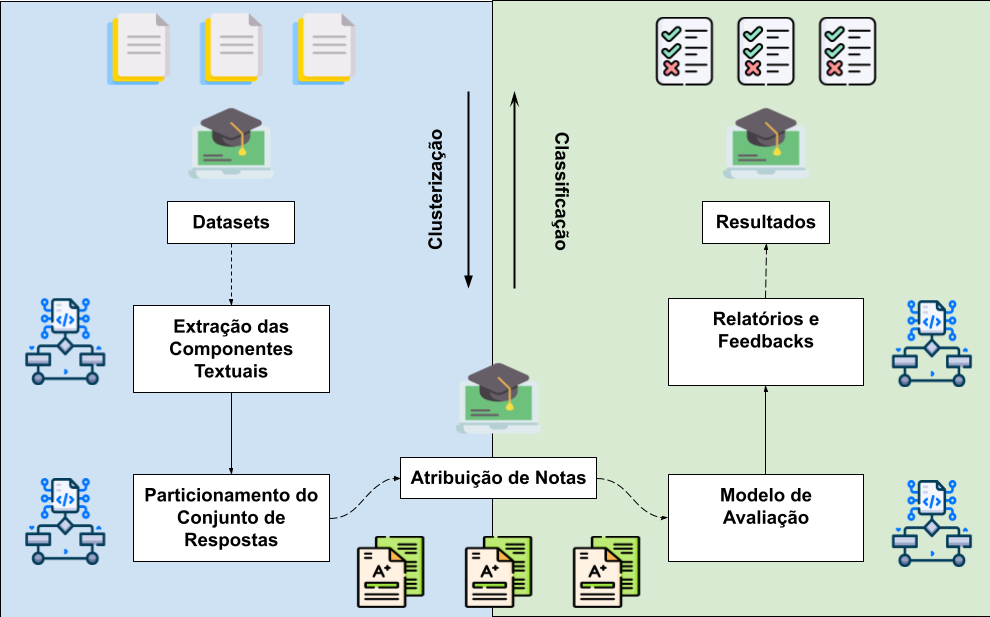
\includegraphics[width=\textwidth]{figuras/estrutura-pNota.png}
\caption{Esquema do \textit{p}Nota dividido em seus quatro módulos.}
\label{fig-esquema}
\end{figure}


Desse modo, tal qual ilustrado na Figura \ref{fig-esquema}, o sistema é composto por quatro módulos. Além destes, outros três processos dependem do estado do documento na avaliação. O primeiro módulo é a \textit{Extração das Componentes Textuais}, que realiza os ciclos de coleta de dados, verificação textual, extração da informação e organização do conhecimento. Nesse módulo o sistema analisa cada resposta com aplicação de tratamentos textuais para padronização e aquisição de conhecimento. O resultado dessa etapa é um conjunto de vetores de documentos com múltiplos níveis de análise da linguagem empregada.

O segundo módulo é composto pelas técnicas de \textit{Particionamento do Conjunto de Respostas}. Nesse núcleo são empregados métodos de otimização em \textit{clustering} para uma seleção representativa do conteúdo textual. Tais técnicas são descritas em detalhes na Seção \ref{sec-amostragem}. A representação criada pelas amostras é o que define o aprendizado do sistema. Por conta disso, as amostras são escolhidas pela sua distribuição espacial \cite{salton1975, baeza2011}, buscando incluir todos os tópicos abordados no tema da questão. Aqui, aplicam-se técnicas de otimização selecionando o agrupamento com melhor desempenho nos índices qualitativos. 

A próxima etapa recebe as atividades particionadas em \textit{clusters} e com a atribuição de notas nas amostras selecionadas. Neste terceiro módulo, com a construção dos \textit{Modelos Avaliativos}, é realizada a calibração dos classificadores e a atribuição das demais notas. A calibração dos algoritmos busca refinar o critério avaliativo para compreender qual é a relação entre os termos e a nota resultante. Ao fim dessa etapa, as notas geradas colaborativamente entre professor e sistema são encaminhadas aos alunos.

Quando os resultados estão prontos, o sistema atua na etapa de \textit{Relatórios e Feedbacks}. Nesse ponto, todas as notas já foram atribuídas e é possível atuar na transparência do modelo avaliativo. Assim, com o conjunto de informações utilizadas durante os processos, são produzidos relatórios e \textit{feedbacks} que descrevem as notas atribuídas e os resultados do \textit{dataset}. Por fim, os relatórios proporcionam acesso ao formato da amostragem, distribuição de notas, análise de desempenho e descrição dos padrões de resposta. 

Antes da execução do sistema, existe a aplicação em sala de aula. Por meio dos AVA, o \textit{p}Nota busca acompanhar a evolução das salas de aula digitais, com o \textit{Ensino a Distância} (EAD) e a disseminação dos MOOCs \cite{mohapatra2017}. Para isso, utiliza-se um \textit{framework} de coleta para transferência e controle das atividades da sala virtual para processamento externo \cite{spalenza2018}. Portanto são responsabilidades da aplicação a coleta das atividades no ambiente virtual, a transferência para um servidor de processamento e o envio de resultados para o professor. Na Figura \ref{fig-framework} é apresentado o funcionamento do método de coleta de dados em diferentes plataformas de ensino.

\begin{figure}[!h]
\centering
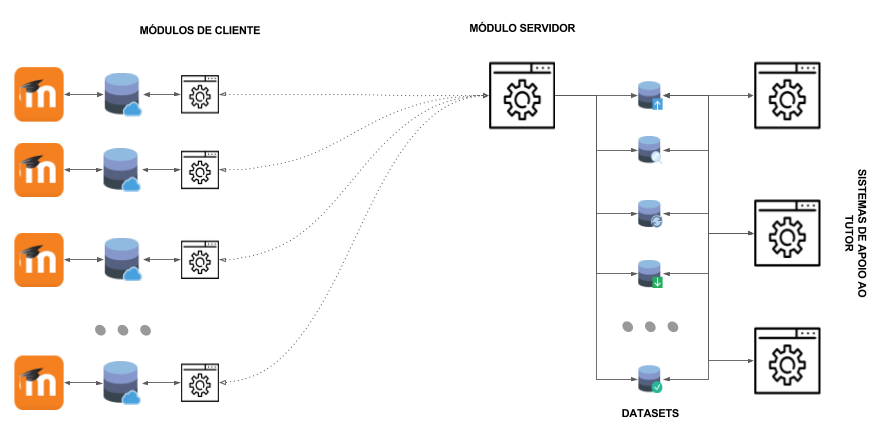
\includegraphics[width=\textwidth]{figuras/framework-moodle.png}
\caption{\textit{Framework} utilizado para transferência de dados, interligando plataformas AVA e o servidor do \textit{p}Nota.}
\label{fig-framework}
\end{figure}

Na Figura \ref{fig-framework} é apresentada a forma empregada na extração de informação dos AVA. Com a configuração, o módulo acessa cada cliente e transfere as atividades para o servidor de processamento do \textit{p}Nota. Então, o \textit{p}Nota solicita via AVA as requisições de avaliação e, após os resultados, também envia as notas para a plataforma. Adicionalmente, os \textit{feedbacks} gerados também são encaminhados individualmente a cada aluno. Na plataforma, após a apresentação das notas, o professor também pode realizar os ajustes necessários caso o resultado não esteja totalmente alinhado ao seu critério.

O professor, controla via plataforma o processamento, sendo aberto para determinar a finalização da atividade diretamente nela. O professor é livre para realizar alterações de qualquer nota mesmo que ainda esteja em análise pelo sistema. No controle do processo avaliativo, o professor fica responsável por monitorar a atribuição de notas e ajustar os resultados propostos pelo sistema.


\section{Extração das Componentes Textuais}
\label{sec-componentes-textuais}

A primeira etapa, \textit{Extração das Componentes Textuais}, realiza o carregamento e a análise do conteúdo textual. Inicialmente é realizada a leitura dos dados, carregando o conjunto de respostas que forma a atividade. É fundamental para extração que o arquivo seja recebido da forma como foi escrito pelo aluno na plataforma. Por conta disso, na sequência é realizada uma série de pré-processamentos que efetuam a limpeza destes documentos, com padronização, segmentação, filtragem, transformação e vetorização. O resultado após essa série de processos é a informação extraída, no formato de vetores com as componentes textuais de cada documento. Na Figura \ref{fig-ect} são apresentados os processos que compõem essa etapa.

\begin{figure}[!h]
\centering
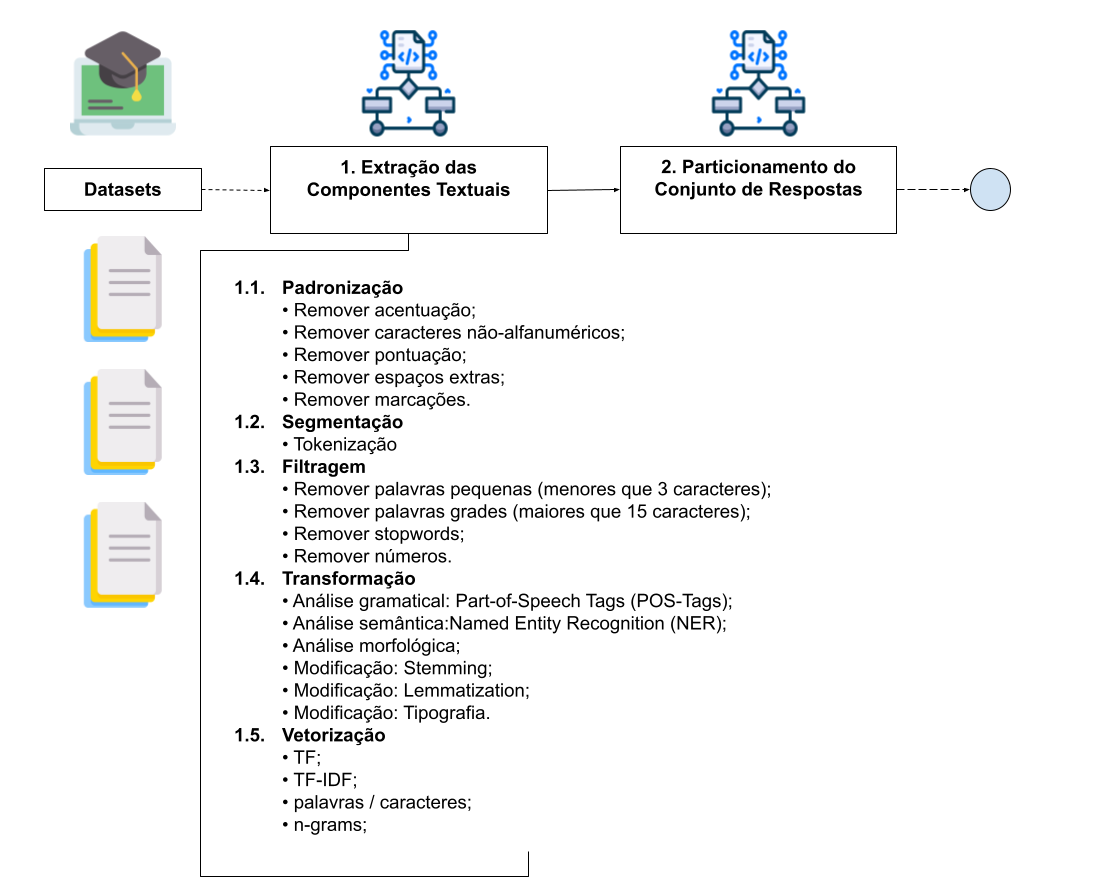
\includegraphics[width=\textwidth]{figuras/esquema-ect-pNota.png}
\caption{Detalhe do módulo de \textit{Extração das Componentes Textuais} no esquema do \textit{p}Nota.}
\label{fig-ect}
\end{figure}

Como é mostrado na Figura \ref{fig-ect}, realizamos todo o tratamento do texto nessa etapa, com coleta das informações. A padronização é composta pela coleta do conteúdo da resposta, remoção de dados não-informativos e aumento da equivalência entre as ocorrências dos termos. A segmentação efetua o particionamento das respostas em segmentos (\textit{tokens}) para verificação de cada termo. Com as frases particionadas, a filtragem seleciona as palavras com maior potencial de ter vínculo com o conteúdo. A transformação realiza análise do conteúdo para aquisição de informação em outros níveis de linguagem. Por fim, com documentos em padrões textuais realiza-se a vetorização, gerando vetores com cada \textit{token} ou série de \textit{tokens} representando o conteúdo enviado pelos alunos.

As respostas, que são recebidas em formato bruto, partem então para pré-processamentos e análises de conteúdo durante essa etapa. Aqui é fundamental a adição dos níveis de compreensão linguística, para amplificar a capacidade de aprendizado dos algoritmos nas próximas etapas. Assim, é pela forma que o texto é passado no formato vetorial \cite{baeza2011} que são identificadas respostas compatíveis até o passo da \textit{Avaliação}.


\subsection{Padronização}
\label{subsec-padronizacao}

% STD_MTH = ["accents", "punct", "spaces", "tags"]

Após o documento ser enviado pelo aluno, o conteúdo do(s) arquivo(s) está em estado bruto. No estado bruto, o conteúdo não segue padrões, em especial de codificação, espaçamento, acentuação e pontuação. É necessário portanto que o formato bruto chegue ao nível de escrita que o aluno enviou ao professor. Além disso, é fundamental remover conteúdos não interpretáveis, como caracteres não alfanuméricos e \textit{tags} (marcações). Portanto, essa etapa é composta pelos seguintes processos:

\begin{itemize}
	\item Remover acentuação;
	\item Remover caracteres não-alfanuméricos;
	\item Remover pontuação;
	\item Remover espaços extras;
	\item Remover marcações.
\end{itemize}

Após cada um dos passos, o texto do aluno está normalizado, tornando possível sua manipulação em nível de conteúdo. Pode-se inferir que a navegação no conteúdo só é possível após a remoção dos ruídos. São usados como exemplos as tags \textit{HTML} e a acentuação. Por um lado, os sinais da linguagem, como acentuação, são fundamentais para leitura e pronúncia dos termos. Mas estes são irrelevantes para identificação dos termos pelo sistema. Por outro lado, o inverso ocorre com marcações de arquivos textuais. São estruturas para leitura do sistema, mas não fazem parte do conteúdo produzido pelo estudante. Em ambos os casos, não existe qualquer relação desses dados com a semântica das respostas, e consequentemente, eles são removidos durante o processo. 

Os ruídos são muito comuns nos textos produzidos na internet, causados pela transferência de arquivos em repositórios externos, \textit{crawlers} ou \textit{web services} \cite{han2011}. Portanto, é a remoção de dados que aproxima a interpretação computacional proposta do envio do estudante na plataforma.

\subsection{Segmentação}
\label{subsec-segmentacao}

% TKN_MTH = ["simple", "word", "regex", "informal"]

Com os documentos passíveis de interpretação, e bem próximos ao que foi enviado pelo aluno, começa-se uma análise detalhada de seu conteúdo. Este é iniciado com o particionamento de cada texto em segmentos menores. A segmentação divide em menores componentes de resposta, seja por caracteres, frases ou parágrafos. Cada particionamento, no entanto, é apenas uma forma de entrada para os procedimentos realizados na sequência. Enquanto parte dos processos faz uso do texto em formato de segmentos de palavras, outros fazem análise contextual, comumente aplicada em formato de segmentos de frase.

É mais comum o formato de segmentos de palavras, denominados \textit{tokens}. Em todos os casos os segmentos são extraídos com base em uma \textit{heurística}, que delimita cada segmento. A \textit{heurística} mais comum para \textit{tokenização} é a divisão pelo espaçamento, eliminando os espaços em branco e considerando as palavras. Porém, esses métodos simples são sujeitos a muitas falhas. Nesses casos, são melhores os métodos construídos especificamente para a linguagem, considerando formas específicas de pontuação e divisões textuais. A \textit{tokenização}, então, é o método que transforma o conteúdo em uma lista de palavras.

A sequência de palavras permite que os próximos níveis trabalhem a perspectiva de cada \textit{token} dessa lista ou de sua vizinhança. Mesmo assim, é muito comum que, durante o processo, o documento seja manipulado de diferentes formas, inclusive passando várias vezes pela transformação de texto em lista de \textit{tokens} e vice-versa. Nesse formato, os \textit{tokens} permitem que haja navegação pelos termos adjacentes tal qual a análise dos termos de forma independente.


\subsection{Filtragem}
\label{subsec-filtragem}
% FLT_MTH = ["smallwords", "stopwords", "largewords", "numerals"]


A filtragem de conteúdo é uma componente muito importante desse processo. Apesar de ser uma etapa que causa perda na informação inicial dos \textit{sets} de resposta, a proposta é identificar \textit{features} que adicionam pouco ou nenhum dado relevante. É esperado, que a inerente perda de informação cause melhoria na consistência e na equivalência entre os documentos. Guiada pelo sistema, a limpeza representa itens que têm baixa correlação com o tema, não sendo componentes do núcleo das respostas. Assim, podemos incluir os seguintes componentes como parte desse processo:

\begin{itemize}
	\item Remover palavras pequenas (menores que três caracteres);
	\item Remover palavras grandes (maiores que 15 caracteres);
	\item Remover \textit{stopwords};
	\item Remover números.
\end{itemize}

Com a filtragem, busca-se uma avaliação fortemente ligada ao tema e o emprego contextualizado. É necessário remover os demais termos, que seriam de baixa significância, pouca capacidade de interpretação e menor relação com o que conteúdo. Esse é o caso das \textit{stopwords}. As \textit{stopwords} são palavras que são empregadas na linguagem como conectivos e não estão conectadas com o conteúdo passado. Elas são extremamente importantes para a nossa interpretação e reconhecimento de contexto, mas não adicionam informação quando empregadas. Assim, a lista de \textit{stopwords} é composta por palavras fundamentais para a linguagem durante a comunicação, mas sem potencial para a análise do contexto.

No caso do tamanho das palavras ainda há uma situação adicional para além da aderência ao tema. A filtragem garante que possíveis ruídos que escaparam dos processos anteriores sejam removidos. Casos específicos como caracteres isolados, links e problemas de segmentação na origem podem gerar ruídos ainda nessa parte. Inclusive, sem uma análise matemática complexa, a verificação numérica também entra em boa parte desses casos e pode ser incluída na filtragem. Mas é importante reconhecer os impactos quando os filtros são aplicados. O filtro numérico, por exemplo, afeta diretamente a capacidade de análise de conjuntos de respostas compostas por valores ou datas. 

Uma dificuldade, entretanto, é quantificar qual é o nível de filtragem desejável, balanceando a aquisição da informação. O ideal é que todos os processos de filtragem não causem impacto nos núcleos da resposta, que contêm os termos essenciais e fortemente vinculados ao tema. Nessa linha, em sua maioria, os casos de filtragem de algumas palavras específicas não impactam a forma e mantêm os termos com aderência ao tema.

Nessa etapa, os filtros de conteúdos são métodos de redução de ruído, responsáveis por discernir quais termos podem ser extraídos de cada item de resposta. Os ruídos podem causar a queda no desempenho do algoritmo da mesma forma ou pior do que a perda de informação causada na filtragem. Assim, o ruído em meio ao texto pode ser um grande problema para o sistema durante a interpretação do conhecimento. Com isso, esperamos que a filtragem auxilie os processos subsequentes com a capacidade interpretativa e relacional entre as respostas na formação do \textit{Modelo Avaliativo}.


\subsection{Transformação}
\label{subsec-transformacao}
% TRF_MTH = ["NER", "MORPH", "POS", "STEMM", "LEMMA"]

As análises de conteúdo são realizadas assim que os níveis anteriores prepararam o texto. Na transformação, a linguagem é analisada em níveis linguísticos. Neste processo, são interpretados alguns detalhes da construção textual para extração de \textit{features} via técnicas de NLP. Essas técnicas observam, entre as funções de cada palavra no texto, aspectos desde sua formação até sua função dentro da frase. Os diferentes níveis analisados nessa etapa são apresentados a seguir:

\begin{itemize}
	\item Modificação: Tipografia;
	\item Modificação: \textit{Stemming};
	\item Modificação: \textit{Lemmatization};
	\item Análise Gramatical: \textit{Part-of-Speech Tags} (POS-Tags);
	\item Análise Semântica:\textit{Named Entity Recognition} (NER);
	\item Análise Morfológica;
\end{itemize}

Cada uma das técnicas da lista aplica uma diferente transformação no texto. A primeira, bem simples, realiza a conversão do texto para uma tipografia comum, seja ela com letras maiúsculas ou minúsculas. Por outro lado, \textit{stemming} realiza conversão mais complexa, recuperando a raiz da palavra na construção da linguagem. Com \textit{stemming}, as palavras são convertidas para um núcleo comum, removendo as flexões, os prefixos e os sufixos. Por outro lado, um método equivalente é realizado com \textit{lemmatization}. Nesse outro, as palavras são convertidas para o \textit{lemma}, a palavra base, na forma com a qual é encontrada nos dicionários \cite{baeza2011}. 

Os métodos analíticos compõem ainda outras três formas mais robustas de identificação linguística. A técnica de \textit{POS-Tags} aplica a extração da função gramatical de cada palavra segundo seu emprego na frase. Em âmbito gramatical, identifica-se qual é o papel de cada palavra no contexto, entre verbos, adjetivos, pronomes, totalizando 17 categorias \cite{marneffe2021}.

Em nível semântico, aplica-se \textit{NER}, classificando o tipo de entidade nomeada de cada um dos \textit{tokens}. Com o NER, os nomes encontrados no texto são caracterizados pela classe que eles representam \cite{pirovani2019}. Entre as categorias reconhecidas há \textit{pessoa} (PER), \textit{local} (LOC), \textit{organização} (ORG) e \textit{diversos} (MISC). Isso permite que o sistema reconheça de forma simétrica diferentes menções dentro do conjunto de respostas para as principais categorias de entidades.

Por fim, o analisador morfológico identifica características da construção de cada palavra. Pela análise morfológica, as palavras são representadas pela sua flexão. Entre as flexões classificadas por cada termo estão as nominais (como gênero, número e definição) e verbais (pessoa, modo, tempo, voz). Além disso, esse mesmo processo também é responsável por algumas classificações léxicas de pronomes, adjetivos e advérbios \cite{marneffe2021}.

Cada uma dessas transformações é realizada para ampliar o conhecimento de cada \textit{token}. As análises mais complexas da linguagem e as categorizações dos termos permitem que as respostas sejam interpretadas de forma mais profunda. Essa profundidade é necessária para que, além do nível textual, a simetria das respostas seja levada em consideração. Desse modo, nesse ponto, a linguagem torna-se mais próxima da compreensão do algoritmo do que da forma original, aplicada na escrita.

A resultante desses processos é uma forte análise das componentes textuais de cada documento, buscando a identificação e a compreensão das estruturas textuais \cite{spalenza2020}. Com maior profundidade textual, espera-se tornar o sistema mais flexível para lidar com texto livre \cite{ding2020}. Assim, apesar das nuances da linguagem, o sistema consegue reconhecer e lidar com padrões que estão na composição de cada sentença \cite{filighera2020}. Então, a compreensão de diferentes níveis linguísticos é fundamental para a construção do SAG \cite{sahu2020}.


\subsection{Vetorização}
\label{subsec-vetorizacao}

A vetorização, como última etapa do pré-processamento, é responsável por extrair o modelo numérico de cada documento, permitindo mensurar a diferença ou a equivalência para os demais da coleção. Dessa forma, os documentos são representados por vetores numéricos segundo seu padrão de características. Cada uma das \textit{features} é analisada conforme sua frequência de ocorrência em cada documento do \textit{dataset}. A representação vetorial numérica de cada documento pela frequência é denominada \textit{Term Frequency} (TF). Sendo a coleção de documentos $ D = \{ d_{0}, d_{1}, d_{2}, \hdots d_{i} \} $ e as \textit{features} encontradas nos documentos $ F = \{ f_{0}, f_{1}, f_{2}, \hdots f_{j} \} $.  Portanto, para cada documento $ d $ na coleção $ D $, conta-se a frequência de cada \textit{feature} $ f_{j} $ do vocabulário $ F $. Assim, a forma vetorial do documento de índice $ i $ é dada por $ d_{i} $, sendo o vetor composto pela frequência $ n $ de cada \textit{feature} no documento $ n_{i, j} $. Então, cada documento é representado em $ D $ por sua forma vetorial $ d_{i} = [\ n_{i, 0}, n_{i, 1}, n_{i, 2} \hdots n_{i,j} ]\ $, usando TF.

Dadas as diferenças entre a frequência de cada termo em cada documento, é aplicada a ponderação para equilibrar a relação de frequência. A ponderação é denominada \textit{Inverse Document Frequency} (IDF). O \textit{Term Frequency-Inverse Document Frequency} (TF-IDF) estabelece a relação de que termos que ocorrem em muitos documentos têm menor relevância \cite{baeza2011}. A ponderação ocorre conforme a Equação \ref{eq-tfidf}.

\begin{equation}
TF-IDF = d_{i,j}* \log \frac{n_{D}}{n_{d_{j}}}
\label{eq-tfidf}
\end{equation}

O IDF é uma ponderação na frequência de cada \textit{feature} no vetor $ d_{i, j} $, segundo o total de documentos $ n_{d_{j}} $ que contém $ f_{j} $ em relação ao total de documentos da coleção $ D $. Essa ponderação reduz a diferença numérica entre uma \textit{feature} encontrada em todos os documentos para as \textit{features} que estão apenas em grupos específicos de documentos. Assim, o uso dessa forma potencialmente delimita melhores características (\textit{features}) para a construção de modelos avaliativos. A aplicação desse modelo está associada à capacidade de identificação de características com alta correlação a grupos específicos de nota.

No método de vetorização, durante a contagem de frequência de cada \textit{feature}, é priorizada a análise de vizinhança entre os termos. Preservando o aspecto textual, os \textit{n-grams} estabelecem a frequência conjunta dos termos dentro de sequências. Em vez de cada documento ser representado por um vetor simples da frequência de cada \textit{feature}, essa frequência é calculada segundo a sequências dos $ n $ termos. Sendo assim, aplicamos valores de $ n $ entre 1 a 5-\textit{grams}. São utilizadas simultaneamente as sequências de um a cinco termos, de forma a capturar o comportamento das estruturas textuais na formação dos documentos. Dessa forma, os padrões identificados em \textit{n-grams} \cite{spalenza2020} visam à associação entre \textit{features} fortemente correlacionadas nos vetores, compondo o modelo avaliativo.


\section{Particionamento do Conjunto de Respostas}
\label{sec-amostragem}

No formato vetorial, temos uma representação numérica dos documentos. Por meio dessa representação, podem ser comparadas as estruturas textuais que cada item de resposta contém. A comparabilidade permite identificar o comportamento das respostas definindo padrões. O conjunto desses padrões forma a distribuição das respostas no espaço vetorial. É possível assim, mensurar a proximidade entre as respostas, enquanto amostras, para formação de \textit{clusters} para análise. Aplicando \textit{Unsupervised Learning}, é realizado o \textit{Particionamento do Conjunto de Respostas} para identificar estruturas textuais similares e contextualizar as diferentes formas de resposta. Essa forma de extração de conhecimento por clusterização é apresentada na Figura \ref{fig-pcr}.

\begin{figure}[!h]
\centering
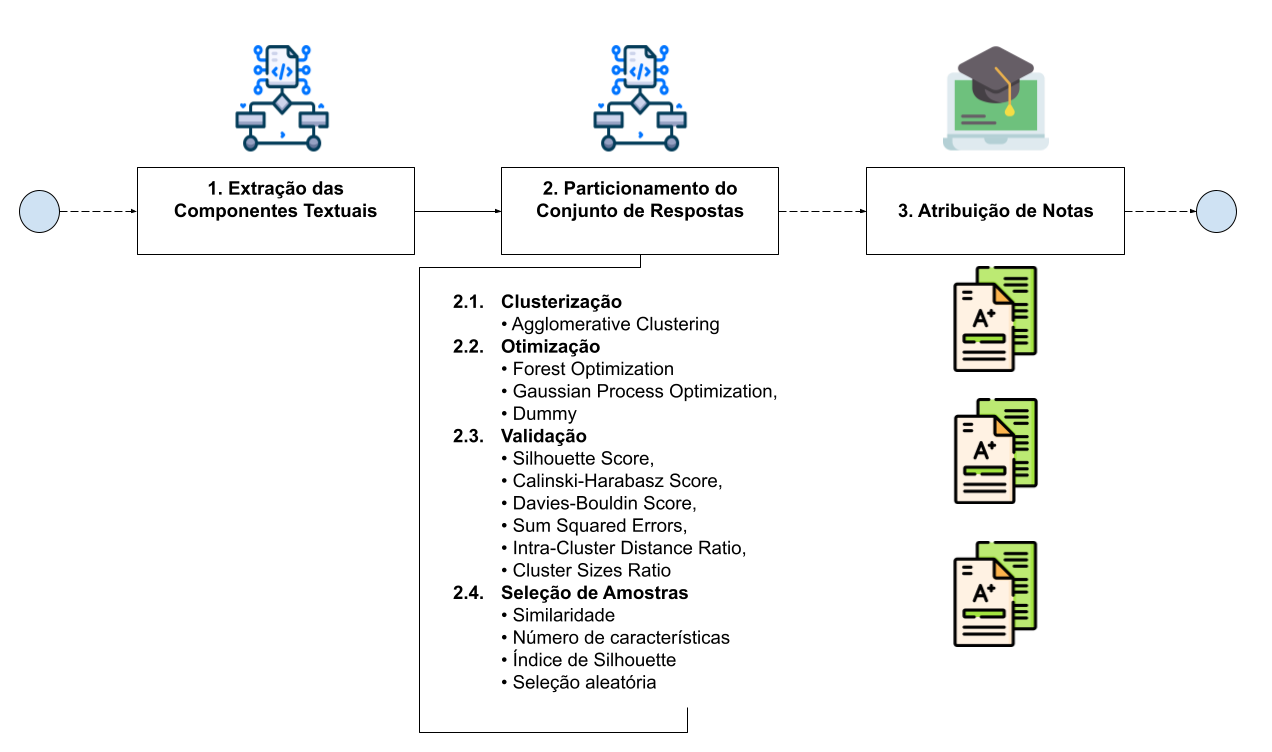
\includegraphics[width=\textwidth]{figuras/esquema-pcr-pNota.png}
\caption{Módulo de \textit{Particionamento do Conjunto de Respostas} no esquema do \textit{p}Nota.}
\label{fig-pcr}
\end{figure}

Na Figura \ref{fig-pcr} é apresentado um primeiro passo do método de \textit{Active Learning} empregado neste trabalho. São identificados diferentes componentes de resposta pela distribuição espacial dos vetores para anotação de amostras selecionadas do conjunto pelo especialista. A partir dessa forma de amostragem, são coletadas as notas, de acordo com o conteúdo que forma cada resposta ou grupo de respostas. Consequentemente, o processo de anotação requisitado pelo sistema vincula o conteúdo destas respostas com os padrões de avaliação do especialista. Diferentemente da maioria dos sistemas, que realizam amostragem aleatória, o \textit{p}Nota analisa as instâncias que compõem cada \textit{cluster} formado.


\subsection{Clusterização}
\label{subsec-clusterizacao}

É realizado o particionamento das respostas utilizando técnicas de clusterização. Esse processo é responsável por agrupar respostas em grupos por similaridade. O algoritmo de \textit{clusterização} utilizado é o \textit{Agglomerative} \cite{spalenza2019}, um método hierárquico de agrupamento por proximidade. O \textit{Agglomerative} compreende formar \textit{clusters} agrupando item a item até que um limiar de proximidade seja alcançado dado um $ k $ número de \textit{clusters} \cite{everitt2011}. Os grupos formados, ou \textit{clusters}, indicam algum nível de compatibilidade entre as estruturas que formam as respostas. Assim, a análise entre a equivalência e a divergência das respostas permite a contextualização da avaliação do especialista.

Para isso, precisamos que os \textit{clusters} sejam bons descritores do contexto, captando bem esse aspecto de equivalências e divergências textuais. A forma de designar se há o equilíbrio entre os \textit{clusters} foi realizada por meio do \textit{elbow method} \cite{everitt2011}. Esse método compreende testar uma sequência de parâmetros da clusterização para identificar a melhor combinação de \textit{clusters} formados segundo uma métrica de qualidade. Em geral, a métrica de qualidade é diretamente relacionada ao propósito de uso dos \textit{clusters}.

Entre as métricas estudadas estão \textit{Calinski-Harabasz Score} (CHS) \cite{calinskiharabasz1974}, \textit{Davies-Bouldin Score} (DBS) \cite{daviesbouldin1979}, \textit{Silhouette Score} (SS) \cite{rousseeuw1987}, \textit{Sum of Squared Errors} (SSE) \cite{maimon2005} e o \textit{Coeficiente de Variação} do tamanho do cluster (CVS). Essas métricas são denominadas \textit{Índices de Validação Interna} e avaliam os agrupamentos sem considerar a classe de cada amostra.

Cada índice é uma heurística utilizada para mensurar, sob diferentes perspectivas, a qualidade dos \textit{clusters} gerados em relação a outras formas de agrupamento de um mesmo \textit{dataset}. CHS mensura a razão entre a dispersão dos itens intra-\textit{cluster} e a dispersão extra-\textit{cluster}. DBS é o índice que estabelece a relação entre a média de similaridade entre as amostras do \textit{cluster} para a média de similaridade entre-\textit{clusters}. SS é a média entre as distâncias das amostras pertencentes a um \textit{cluster} em relação às amostras do \textit{cluster} mais próximo. SSE é uma métrica que avalia o erro de cada amostra que compõe um \textit{cluster} em relação ao seu centroide. O centroide é o ponto médio dos itens que constituem cada \textit{cluster}. Portanto, o centroide é uma instância representante da dispersão dos itens no \textit{cluster}, porém é um ponto artificial e não necessariamente uma amostra que o compõe. Por fim, CVS avalia o equilíbrio entre o número de amostras agrupadas em cada \textit{cluster}, considerando a diferença entre o maior grupo e o menor grupo formados.

Para a avaliação de respostas abertas, consideramos que o ideal são as análises que balanceiam os itens de cada \textit{cluster} em relação aos \textit{cluters} adjacentes. Por isso, \textit{clusters} com padrões muito específicos não devem formar bons descritores para a distribuição, mas sim para uma ou poucas amostras que compõe o grupo. Assim, para a proposta de \textit{Active Learning}, os grupos equilibrados têm maior potencial para aquisição de informação. Por outro lado, também é fundamental reconhecer a proximidade intra e inter-\textit{cluster}. Assim, foram combinados CVS e SS para avaliação amostral. Aplicamos CVS na formação dos agrupamentos enquanto o SS é observado durante a seleção amostral.


O processo de otimização, que incide sobre o \textit{elbow method}, testa os parâmetros de clusterização e visa reduzir o intervalo de busca enquanto maximiza os resultados do índice. Para isso, foram avaliados três métodos \textit{Forest Optimization}, \textit{Gaussian Process Optimization} e \textit{Dummy}. Os resultados obtidos com os dois primeiros foram equivalentes nesse contexto, sendo escolhido o \textit{Gaussian Process} para a aplicação \cite{spalenza2019}. Esse método analisa cada teste pela distribuição dos valores da métrica de qualidade como uma \textit{gaussiana}, buscando pontos de máxima da função. A resultante é dada pelo melhor valor encontrado. O parâmetro sob controle é o $ k $, número de \textit{clusters}. O intervalo de $ k $ é definido por valores de $ 2 $ até $ 2 * \sqrt{n} $, sendo $ n $ o número de amostras do \textit{dataset} \cite{han2011}. Simultaneamente, para cada combinação de $ k $ são testadas 20 métricas de distância.

\begin{itemize}
\begin{multicols}{4}
  \item braycurtis
  \item canberra
  \item chebyshev
  \item correlation
  \item cosine
  \item dice
  \item euclidean
  \item hamming
  \item haversine
  \item jaccard
  \item kulsinski
  \item mahalanobis
  \item manhattan
  \item matching
  \item minkowski
  \item rogerstanimoto
  \item russellrao
  \item sokalmichener
  \item sokalsneath
  \item yule
  \end{multicols}
\end{itemize}

O agrupamento selecionado é utilizado para amostragem em um percentual do conjunto de respostas disponíveis. Ainda avaliamos de forma qualitativa essa seleção segundo três índices \textit{Homogeneity} (HS), \textit{Completness} (CS) e \textit{Clustering Accuracy} (CA). Em uma ótica diferente da formação dos \textit{clusters}, com os índices qualitativos é mensurado o impacto de cada resultado da clusterização pela distribuição das classes. Esses são chamados \textit{Índices de Validação Externa}.

CA é o índice que avalia o desempenho da clusterização enquanto classificador por voto majoritário. Nesse cenário, cada \textit{cluster} é representado pela sua principal classe, mostrando a coesão dos grupos para sua representação de classe. Esse índice também estabelece um \textit{baseline} de desempenho de classificação. Essa métrica é simétrica a ACC, descrita na Equação \ref{eq-classification} da Seção \ref{subsec-classificacao}. HS é o índice que mensura se os \textit{clusters} são formados apenas por uma classe \cite{rosenberg2007}. CS por outro lado, avalia se todos os itens de uma classe estão presentes em um mesmo \textit{cluster} \cite{rosenberg2007}. Ambos são métricas que avaliam a entropia ($H$) dos \textit{clusters} dada a anotação das amostras, apresentadas na Equação \ref{eq-hs-cs}.

\begin{equation}
Homogeneity = 1 - \frac{H(y_{c} | \hat{y}_{c})}{H(y_{c})}
\label{eq-hs-cs}
\end{equation}

\begin{equation*}
Completness = 1 - \frac{H(y_{c} | \hat{y}_{c})}{H(\hat{y}_{c})}
\end{equation*}

A Equação \ref{eq-hs-cs} apresenta as métricas HS e CS, referências para a concentração das classes reais ($y_{c}$) dada a distribuição dos \textit{clusters} ($\hat{y}_{c}$). Assim, identifica-se o comportamento das classes de nota na distribuição pela entropia. Tais métricas permitem a identificação \textit{a posteriori} dos resultados mais coesos de clusterização. A concentração de classe por \textit{cluster}, permite uma melhor amostragem sendo possível amplificar os resultados obtidos na etapa de classificação.


\subsection{Seleção de Amostras}
\label{subsec-selecao-amostras}

Com a formação dos \textit{clusters}, identificam-se as principais respostas de cada agrupamento para inferência do modelo avaliativo do professor. A amostragem é realizada com a coleta de um percentual dos itens mais representativos que compõem o \textit{dataset}. Essa coleta analisa padrões de documentos de cada \textit{cluster}, a fim de compreender como é dada a avaliação do especialista para os diferentes padrões de resposta. As amostras são selecionadas conforme critérios específicos, descrevendo componentes do \textit{cluster}. 

A nossa amostragem segue alguns critérios. Os critérios definem a sequência de seleção para atingir o percentual escolhido para anotação. No primeiro grupo de amostras são selecionados os pares de amostras que apresentam maior e menor similaridade de cada \textit{cluster}. O segundo grupo é composto por amostras com mais e menos características. O terceiro grupo é formado de duas formas: pelo coeficiente \textit{silhouette} \cite{rousseeuw1987} de cada amostra ou pela seleção aleatória.

Nesse último grupo a análise de dispersão calcula o coeficiente de \textit{silhouette} da amostra. Tal qual o SS, esse índice determina a razão entre a distância da amostra para os demais itens do grupo em relação aos itens do \textit{cluster} mais próximo. Dessa forma, por meio desse método é incrementado o número de amostras por dispersão até alcançar o percentual de amostragem selecionado. Uma outra opção de seleção é a escolha de amostras pelo balanceamento do tamanho dos \textit{clusters}. Nesse caso, o método determina que um item seja aleatoriamente selecionado, ponderado de acordo com a quantidade de itens que compõem cada grupo. Descartando as duas opções anteriores, as amostras são selecionadas aleatoriamente entre todo o \textit{dataset}.

Terminando esse procedimento de seleção, as amostras são enviadas para atribuição de notas pelo professor. Na plataforma de correção que o professor adotou, ele realiza a atribuição de notas para cada item sugerido pelo sistema após a amostragem. Finalizado esse processo, com o conjunto de respostas representativas e suas respectivas notas atribuídas pelo professor, começa-se a análise de padrões para inferência das notas para as demais respostas.

\section{Modelo Avaliativo}
\label{sec-avaliacao}

O passo posterior à atribuição de notas, etapa com participação do professor, é a criação dos modelos computacionais. O \textit{Modelo Avaliativo}, é a etapa do \textit{p}Nota que desenvolve o SAG para replicar a forma de avaliação do professor. Assim, após a atribuição de notas, são criados os padrões que vinculam o texto e a avaliação.  O sistema, portanto, deve se aproximar da forma como o professor gera avaliações. A plataforma utilizada para reconhecimento de padrões de nota é apresentada na Figura \ref{fig-ma}.

\begin{figure}[!h]
\centering
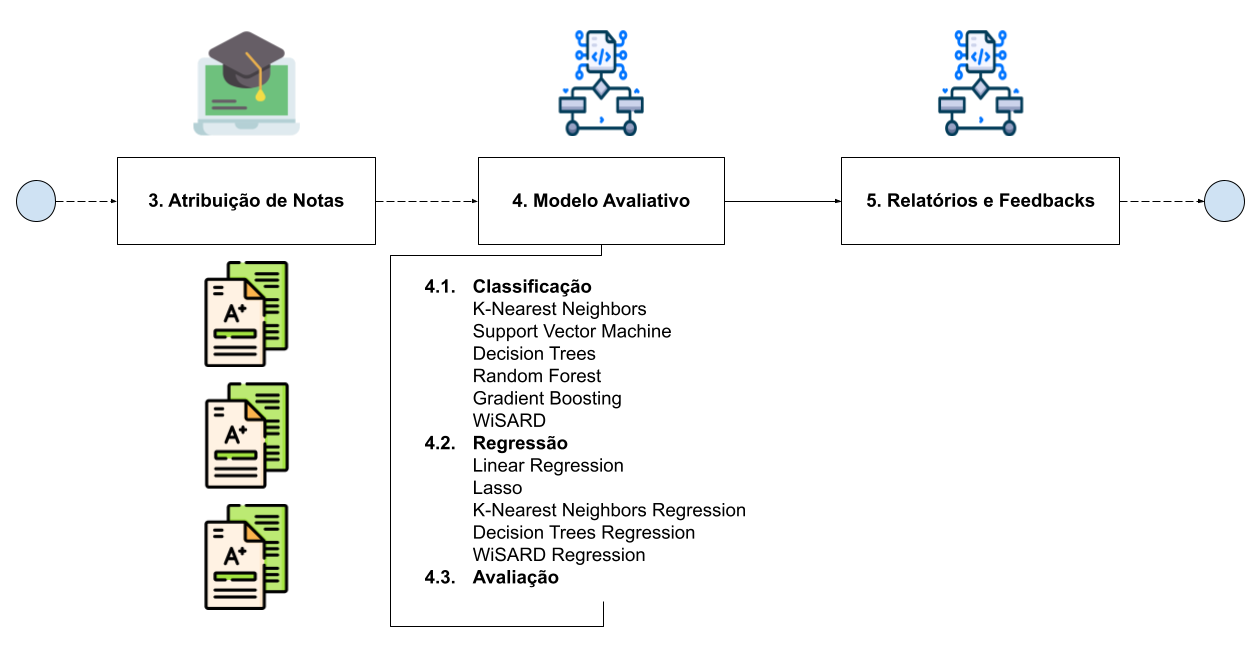
\includegraphics[width=\textwidth]{figuras/esquema-ma-pNota.png}
\caption{Etapa de construção do \textit{Modelo Avaliativo} no esquema do \textit{p}Nota.}
\label{fig-ma}
\end{figure}

Ao receber todas as notas para as amostras, o processo começa a construção dos modelos, tal qual ilustrado na Figura \ref{fig-ma}. A criação de um modelo SAG complexo compreende identificar detalhes correspondentes entre as respostas. O \textit{p}Nota analisa a correspondência entre notas e \textit{features} textuais para analisar equivalência. É possível considerar que padrões equivalentes de uma mesma nota têm alta probabilidade de serem relacionados ao que o professor considerou para avaliação. Cada atividade tem especificamente uma forma de avaliação e um padrão avaliativo alinhado com a prática do professor. Portanto, a identificação do critério avaliativo não é trivial. Por isso, a técnica de \textit{Active Learning} proposta neste estudo é fundamental para compreender o modelo e a forma que o professor trabalha durante a avaliação.

O \textit{Modelo Avaliativo} gerado pelo \textit{p}Nota é responsável por atender a expectativa de nota do professor. Sua função é vincular o padrão avaliativo com o padrão textual (\textit{features}) do conjunto de resposta. Então, a função da técnica de \textit{Active Learning} proposta é treinar classificadores contextuais, transformando os métodos tradicionais de ML em avaliadores especializados. Por meio do conhecimento de uma série de níveis de linguagem e da otimização da seleção de amostras busca-se reduzir os problemas que são incorretamente atribuídos apenas à técnica aplicada na atribuição de notas. Desta forma, espera-se que os \textit{Modelos Avaliativos} lidem com a variação linguística, a individualidade dos \textit{outliers} e o desbalanceamento dos níveis de nota.


\subsection{Classificação}
\label{subsec-classificacao}

O processo de classificação é utilizado em dois tipos distintos de avaliação: com notas ordinais e discretas. As notas ordinais permitem estabelecer ordem de escala numérica enquanto as discretas são textuais e requerem interpretação. No entanto, aos classificadores empregados, trabalha-se com a relação de diferença entre os níveis para aprendizado de convergência e divergência. Por um lado, a convergência indica equivalência entre os padrões de avaliação e texto encontrados nas amostras. Por outro lado, a divergência indica os padrões incompatíveis de texto por nota e entre níveis de nota, degradando sua influência avaliativa. As técnicas empregadas, em sua essência, devem assimilar o que compõe um nível de nota (equivalência) e o que é informação irrelevante ou auxiliar (divergência). Para estudar esses aspectos são aplicadas cinco diferentes formas de reconhecimento de padrões por meio dos algoritmos: \textit{K-Nearest Neighbors}, \textit{Decision Tree}, \textit{Support Vector Machine}, \textit{Gradient Boosting}, \textit{Random Forest} e \textit{WiSARD}.

O \textit{K-Nearest Neighbors} (KNN) é o algoritmo de classificação pela análise da vizinhança amostral. No KNN, cada amostra é categorizada pela distribuição local dos seus $ k $ vizinhos. A atribuição do rótulo é por voto majoritário, atribuindo o mesmo valor à amostra não anotada. Diferentemente deste, o algoritmo \textit{Decision Tree} (DTR) estabelece a equivalência entre amostras, sob uma perspectiva das características que as compõem. O DTR associa os grupos anotados com a mesma classe pelos limiar das características, gerando regras de decisão. As regras, elaboradas automaticamente, delimitam as principais \textit{features} segundo os valores de tendência de classe. O processo de classificação, então, acontece com a comparação de cada um dos itens dentre a cadeia de decisões na estrutura de árvore.

Outro tradicional algoritmo, o \textit{Support Vector Machine} (SVM) estabelece uma forma distinta de observar os dados. Os dados, em grupos por categoria, formam um \textit{kernel}. O \textit{kernel}, diferentemente do DTR, cria modelo espacial que delimita a diferença entre categorias. Então, cada amostra, é identificada segundo sua posição em relação ao limiar de características dado o modelo representante da classe. De forma similar é aplicado o algoritmo \textit{Wilkes, Stonham and Aleksander Recognition Device} (WSD) \cite{aleksander1984, wisard2020}, conhecido como \textit{WiSARD}\footnote{wisardpkg - https://github.com/IAZero/wisardpkg}. O algoritmo produz um modelo binário com o registro de padrões de características. Cada padrão é reconhecido em análise sequencial de um intervalo de bits predefinido. O modelo binário criado é comparado com as respostas não avaliadas, categorizando-as pela similaridade entre padrões. Especificamente para esse algoritmo, a conversão dos vetores TF-IDF em seu formato binário foi dada com 1 \textit{bit} por característica, de acordo com a esparsidade observada em dados textuais \cite{manning1999}. Assim, dado como pré-requisito de sua aplicação, o padrão submetido é dado pela existência (valor 1) ou não (valor 0) de cada característica na resposta.

Adicionalmente, dois modelos de \textit{ensemble} foram aplicados. Os \textit{ensembles} são técnicas que combinam vários classificadores mais simples para determinar áreas de decisão mais robustas. Os classificadores simples são denominados \textit{weak learners}, em busca de detalhes na avaliação entre termos e classes. Nesse aspecto, \textit{Random Forest} (RDF) é um algoritmo que combina o método tradicional \textit{Decision Tree} com \textit{subsets} de amostras. Desta forma, o RDF combina análises parciais do conjunto de dados para definir regras de decisão mais complexas sobre a distribuição de amostras. De modo similar, o \textit{Gradient Boosting} (GBC) combina uma série de \textit{Regression Trees} para otimização diferencial da função de perda (\textit{loss}). Nessa linha, o GBC observa o gradiente da função de perda com \textit{Logistic Regression}. Nesse aspecto, com uma série de amostragens, a técnica procura minorar o erro de classificação obtido com a calibração do modelo segundo uma sequência de \textit{subsets}. 

A combinação com modelos tradicionais e técnicas de \textit{ensemble} visa potencializar a capacidade analítica do método. Com diferentes formatos de dados, a proposta deste trabalho testa diferentes modelos procurando o que melhor se adapta ao padrão avaliativo do professor. Nesse aspecto, o método de classificação é escolhido de acordo com a similaridade entre o modelo automático com o critério do professor \cite{pado2021}. Para avaliar esse aspecto utiliza-se o coeficiente \textit{kappa} quadrático \cite{cohen1960}. As amostras são separadas em dois grupos acordo com o \textit{Stratified K-Fold}, para mensurar a capacidade de cada algoritmo na categorização das amostras. Dentro do próprio conjunto utilizado para treinamento dos modelos SAG, é possível avaliar a paridade dos resultados com o avaliador humano \cite{artstein2008}.

Na sequência, a qualidade de cada um é avaliada com quatro métricas. A \textit{Accuracy} (ACC), ou acurácia, mensura a equivalência percentual entre as avaliações. A \textit{Precision} (PRE), ou precisão, quantifica a atribuição correta de rótulos em razão da quantidade de atribuições incoerentes da mesma categoria. De forma similar, a \textit{Recall} (REC), ou revocação, quantifica a atribuição correta de rótulos em razão dos itens de determinada classe que foram classificados de forma incorreta. Por fim, F1 é o balanceamento entre PRE e REC, observando simultaneamente os erros de e para cada classe. A Equação \ref{eq-classification} apresenta a fórmula de cada uma das métricas citadas para avaliação qualitativa dos algoritmos de classificação testados.

\begin{equation}
Accuracy = \frac{TP+TN}{TP+TN+FP+FN}
\label{eq-classification}
\end{equation}

\begin{equation*}
Precision = \frac{TP}{TP+FP}
\end{equation*}

\begin{equation*}
Recall = \frac{TP}{TP+FN}
\end{equation*}

\begin{equation*}
F{1} = \frac{2*Precision*Recall}{Precision+Recall}
\end{equation*}

Na Equação \ref{eq-classification}, é possível observar as fórmulas para mensurar a qualidade dos classificadores. Nelas $ T $ refere-se aos casos verdadeiros e $ F $ aos falsos. Da mesma forma, $ P $ refere-se aos casos positivos e $ N $ aos negativos \cite{manning2008}. Porém, tradicionalmente a avaliação tem nuances que se extendem para além das marcações entre certo (ou verdadeiro) e errado (ou falso). Assim, as métricas são balanceadas conforme o número de classes, como determinado na Equação \ref{eq-classification-nlabels}. 

\begin{equation}
Accuracy = \frac{1}{n_\text{amostras}} \sum_{i=0}^{n_\text{amostras}-1} 1(\hat{y}_i = y_i)
\label{eq-classification-nlabels}
\end{equation}

\begin{equation*}
Precision_{macro} = \frac{1}{\left|n_{classes}\right|} \sum_{c \in n_{classes}} Precision(y_c, \hat{y}_c)
\end{equation*}

\begin{equation*}
Recall_{macro} = \frac{1}{\left|n_{classes}\right|} \sum_{c \in n_{classes}} Recall(y_c, \hat{y}_c)
\end{equation*}

\begin{equation*}
F{1}_{macro} = \frac{1}{\left|n_{classes}\right|} \sum_{c \in n_{classes}} F{1}_\beta(y_c, \hat{y}_c)
\end{equation*}

\begin{equation*}
F{1}_{ponderado} = \frac{1}{\sum_{c \in n_{classes}} \left|y_c\right|} \sum_{c \in n_{classes}} \left|y_c\right| F{1}(y_c, \hat{y}_c)
\end{equation*}

A Equação \ref{eq-classification-nlabels} mostra as métricas qualitativas aplicadas em avaliações com múltiplos níveis de nota, sendo $y$ o valor de nota atribuído para cada amostra ou grupo de amostras ($c$) \cite{manning2008}. Por definição, os SAGs são majoritariamente criados para avaliações com mais de uma classe de nota. É usada para mensurar o desempenho a média (macro) da atribuição de notas. Porém, pelo já esperado desbalanceamento entre notas, também avalia-se o F1 ponderado pela quantidade de amostras por classe. Comparando estatisticamente os desempenhos, via \textit{kappa}, a expectativa é selecionar o que tem notas mais adequadas ao modelo avaliativo do professor. Mas, o melhor modelo é o que efetivamente apresenta maior ganho de qualidade nessas métricas quando comparado com a avaliação final do professor.


\subsection{Regressão}
\label{subsec-regressao}

Outra forma de atribuição de nota é a não-categórica. Nesses casos, são chamadas de notas contínuas, pois apresentam um intervalo de notas possíveis mas sem níveis específicos. São aplicados os métodos de regressão, estimando a nota pela similaridade entre respostas. Nesse formato ainda se enquadram as noções de \textit{equivalência} e \textit{divergência} entre as \textit{features} das respostas na avaliação. Os cinco métodos de regressão aplicados são \textit{Regressão Linear}, \textit{Lasso}, \textit{K-Nearest Neighbors}, \textit{Decision Tree} e \textit{WiSARD}.

A Regressão Linear (LNRG) é um algoritmo que avalia a tendência linear das amostras segundo sua distribuição. Essa tendência linear busca, no espaço n-dimensional das características, definir os coeficientes do hiperplano que minimizam o resíduo entre as amostras. É importante para o algoritmo determinar uma função de tendência dos dados. Minimizar o erro pelos coeficientes da função reflete na simplificação do conjunto de dados. Contudo é determinante que o modelo não apresente \textit{overfitting} e um baixo desempenho com o viés dos dados de treinamento. Por outro lado, como espera-se do algoritmo, a aquisição de informação deve extrair um modelo que minimamente descreva os dados conhecidos, evitando a ocorrência de \textit{underfitting}. Assim, o modelo simplificado deve ser direcionado ao desempenho linear e não apenas à associação forte com o conjunto de treinamento. Também é utilizada uma variante do LNRG tradicional, denominada \textit{Least Absolute Shrinkage and Selection Operator - Lasso} (LSSR), que utiliza a normalização dos dados com a função $ L1 $, reduzindo a complexidade do modelo de dados e prevenindo o \textit{overfitting}.

Os demais três modelos, são similares aos modelos utilizados na classificação. O \textit{K-Nearest Neighbors} (KNRG), assim como o algoritmo de classificação, observa a distribuição dos dados e define o valor resultante de acordo com a vizinhança. Assim, o resultado de cada amostra de valor desconhecido é a interpolação entre os valores das $ K $ amostras mais próximas conhecidas. De forma semelhante, \textit{Decision Tree} (DTRG) observa características semelhantes entre amostras e, por equivalência, divide em subgrupos. A subdivisão dos itens na árvore e o particionamento em subgrupos delimita regiões específicas com resultantes correspondentes por aproximação. Dessa maneira, após o particionamento das regiões amostrais em zonas de decisão, o valor dado para todas as amostras ali categorizadas é a média conhecida do subgrupo de treinamento. De forma similar funciona a WiSARD (WSRG), organizando registradores com as notas das respostas similares atribuindo o valor médio do registrador para respostas de padrão equivalente.

Para seleção do regressor mais adequado utiliza-se a correlação de \textit{Pearson}. Pela correlação mensura-se a compatibilidade dos avaliadores como pares, do sistema e do professor. Nessa visão, maiores índices de correlação indicam distribuições equivalentes de distribuição de notas \cite{morettin2010}. Isso implica modelos avaliativos mais equivalentes ao método avaliativo do professor. Já a avaliação é dada pelo resíduo entre as duas notas, considerando como ideal o modelo que apresenta uma série de notas próximas do que foi atribuído pelo professor. Assim, para mensurar a diferença entre a expectativa do professor e a nota resultante do sistema são utilizadas três métricas: o \textit{Mean Absolute Error} (MAE), o \textit{Mean Squared Error} (MSE) e o \textit{Root Mean Squared Error} (RMSE)

O MAE, erro médio absoluto, mensura a resíduo absoluto entre a nota predita e a nota dada pelo professor. Em outras palavras, o MAE avalia as diferenças em módulo entre os valores obtidos, segundo o alinhamento de cada predição com a expectativa do professor. Enquanto isso, MSE ou erro médio quadrático, é uma medida do resíduo entre os valores com penalização dos erros absolutos. Assim, por meio do MSE erros maiores têm maior impacto no sistema quando comparados com erros de menor grau. Por fim, o RMSE ou raiz do erro médio quadrático, é a raiz quadrada do valor obtido no MSE, normalizando o erro obtido nessa métrica em relação à avaliação do professor. A Equação \ref{eq-regressao} apresenta a fórmula de cada uma das métricas utilizadas para avaliação dos métodos de regressão citados.

\begin{equation}
MAE = \sum_{i=0}^{D}|y_i-p|
\label{eq-regressao}
\end{equation}

\begin{equation*}
MSE = \sum_{i=0}^{D}(y_i-p)^2
\end{equation*}

\begin{equation*}
RMSE = \sqrt{\sum_{i=0}^{D}(y_i-p)^2}
\end{equation*}

Na Equação \ref{eq-regressao} são apresentadas as fórmulas de avaliar o erro do modelo criado conforme a expectativa de nota. Assim, em cada fórmula as amostra $ i $ da coleção são comparadas com as notas atribuídas do avaliador humano (professor) $ y $ e pelo sistema $ p $. O melhor modelo avaliativo é o que apresenta menor nível de erro em relação à atribuição de notas do professor. Apesar de serem comuns os erros entre modelos computacionais e a expectativa do especialista, é crucial para um bom avaliador automático a proximidade entre os modelos. Nos sistemas SAG, foram observados durante a correção entre professores até 0,66 pontos de divergência em notas de zero a cinco pontos \cite{mohler2011}. Em uma escala de zero a dez pontos, representaria 1,32 pontos de divergência entre avaliadores humanos. Assim, é esperado que o sistema minimize os erros em relação ao professor, reduzindo a divergência para a nota do professor.


\section{Relatórios e \textit{Feedbacks}}
\label{sec-relatorios}

Com as notas atribuídas pelo sistema, ocorre a criação de relatórios e \textit{feedbacks}. Eles contribuem para descrição do modelo de Inteligência Artificial aplicado na atribuição de notas. Em especial, os \textit{feedbacks} devem destacar quais são as \textit{features} relevantes levadas em conta na criação do modelo avaliativo. Nessa mesma linha, os relatórios são a forma de descrever os processos realizados para todos os participantes. Esta etapa, aplicada na descrição dos processos internos do \textit{p}Nota, é ilustrada na Figura \ref{fig-rf}. 

\begin{figure}[!h]
\centering
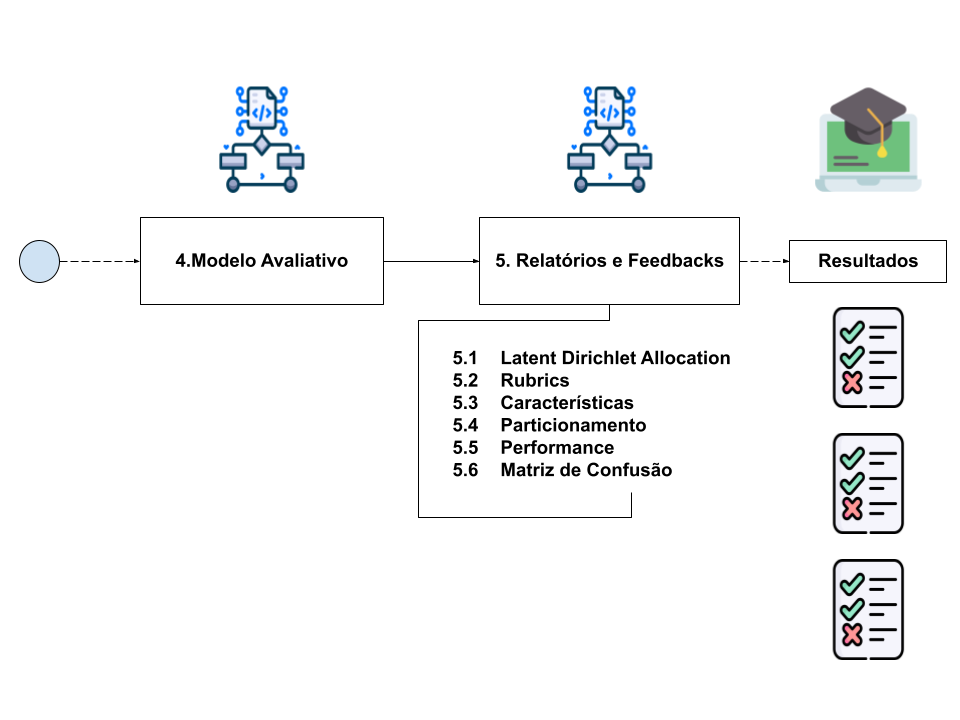
\includegraphics[width=\textwidth]{figuras/esquema-rf-pNota.png}
\caption{Módulo de \textit{Relatórios e Feedbacks} no esquema do \textit{p}Nota.}
\label{fig-rf}
\end{figure}


Conforme a etapa apresentada na Figura \ref{fig-rf}, os relatórios precedem o envio dos resultados para o AVA, de forma a descrever o \textit{Modelo Avaliativo}. Com fundamento na relação entre termos e notas, a caracterização das respostas é determinante para conectar usuários com os métodos aplicados pelo \textit{p}Nota. Assim, os relatórios e os \textit{feedbacks} devem descrever em detalhes a forma de avaliação aplicada para instruir os usuários. Um exemplo completo dos relatórios é apresentado no Apêndice \ref{exemplo-pNota}.

Os procedimentos de descrição do \textit{p}Nota incluem, desde características superficiais, conectadas às calibrações e às etapas do sistema, até características mais profundas, que contextualizam a interpretação do sistema sobre a atividade. É possível citar como exemplos do primeiro os \textit{clusters} formados, amostras selecionadas para anotação ou características mais frequentes. No segundo, por outro lado, são apresentados em linguagem natural os resultados e a proximidade entre as notas.


\subsection{Relatório dos Processos}
\label{subsec-relatorio-processos}

Os relatórios buscam passar por cada etapa do \textit{p}Nota para mostrar como foram as interações com o professor e os resultados obtidos. Um desses é o relatório de esforço de anotação e treinamento do algoritmo. Retomando o exemplo do Capítulo \ref{cap1-intro}, na Tabela \ref{tab-ptasag-train-46} é apresentado tal relatório para a atividade 46 do \textit{dataset PTASAG}.

\begin{table}[!b]
\centering
\caption{Particionamento das amostras em treino e teste na atividade exemplo \textit{PTASAG Atividade 46}.}
\label{tab-ptasag-train-46}
\begin{tabular}{|c c c c|} \hline
\multicolumn{3}{|l}{Dataset} & Amostras\\ 

\multicolumn{3}{|l}{PTASAG : Atividade 46} & 655 \\ \hline 

Treino (Un.) & Treino (\%)  & Teste (Un.) & Teste (\%) \\ \hline 

524 & 80.0 & 131 & 20.0 \\ 

\hline \hline
\end{tabular}
\end{table}


Na Tabela \ref{tab-ptasag-train-46} é apresentado um exemplo de relatório utilizado para explicar o que foi realizado em um dos processos. O mesmo informa qual foi o particionamento de amostras utilizado e qual foi o esforço de correção do professor. Porém, o nível descritivo deve ser maior quando caracterizamos aspectos avaliativos, tornando cada vez mais transparente a avaliação. Durante a elaboração destes, identifica-se uma certa dificuldade de interpretação das métricas categóricas em relação ao observado com métricas contínuas. Por conta disso, são estabelecidos três níveis de desempenho para as métricas percentuais: \textit{Avançado}, \textit{Adequado} e \textit{Insuficiente} \cite{nascimento2020}.

\begin{itemize}
	\item Intervalo de 75\% - 100\%: Nível \textcolor{green}{Avançado};
	\item Intervalo de 35\% - 75\%: Nível \textcolor{yellow}{Adequado};
	\item Intervalo de 0\% - 35\%: Nível \textcolor{red}{Insuficiente}.
\end{itemize}


Os níveis são similares aos que o professor utiliza para determinar o conteúdo assimilado pelos alunos durante a avaliação \cite{nascimento2020}. Em nível \textcolor{red}{Insuficiente} a relação entre as notas finais divulgadas pelo professor e as notas do sistema apresenta índices abaixo do esperado. Em nível \textcolor{yellow}{Adequado} as notas apresentam alinhamento com as que foram atribuídas pelo professor. E em nível \textcolor{green}{Avançado}, os resultados do modelo avaliativo foram próximos aos divulgados pelo especialista, identificando bem seu método avaliativo. Assim, foi necessário trazer para a realidade em sala de aula os resultados da classificação, tal qual já é a realidade quando é aplicado o nível de erro entre avaliadores \cite{almeida-junior2017}. Na Figura \ref{fig-ptasag-performance-46} é apresentado o desempenho de categorização conforme esses três níveis.

\begin{figure}[!t]
 \centering
 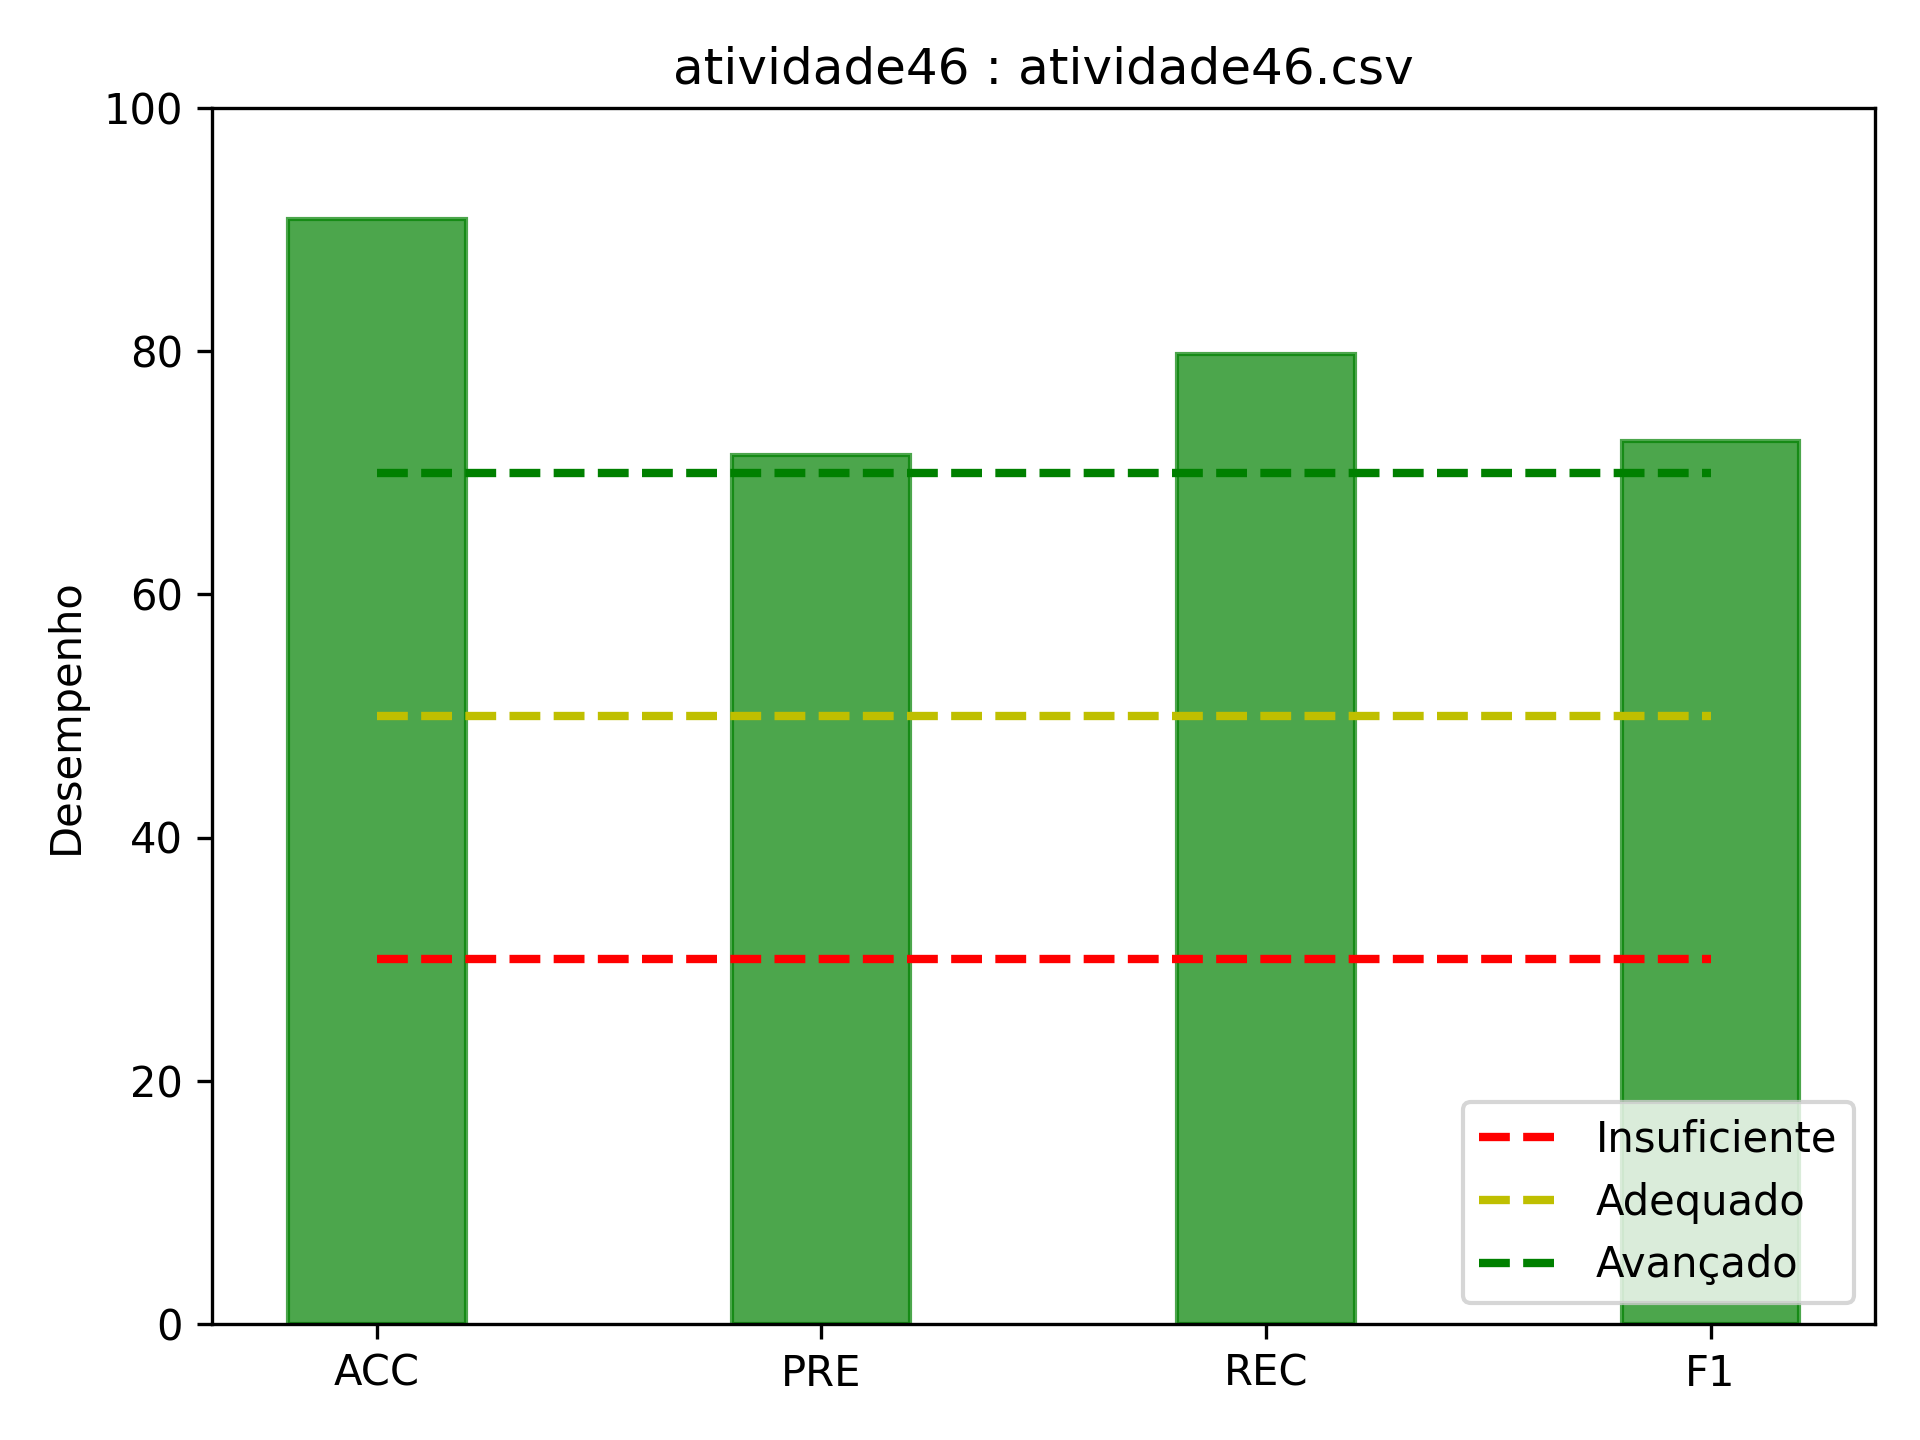
\includegraphics[width=0.8\textwidth]{figuras/exemplo/exemplo-ptasag-rdf.png}
 \caption{Resultados de desempenho do exemplo \textit{PTASAG Atividade 46}.}
 \label{fig-ptasag-performance-46}
\end{figure}

Na Figura \ref{fig-ptasag-performance-46}, há um resultado de alto desempenho de classificação usando o classificador RDF. Com os níveis e as cores, os resultados e as métricas de avaliação tornam-se um pouco mais simples para interpretação e análise dos professores, sendo assim, uma ferramenta útil para comparação e uso na sua rotina de validação do sistema.


\subsection{\textit{Feedbacks} Contextuais}
\label{subsec-feedbacks-contextuais}

Os \textit{feedbacks} contextuais são métodos que descrevem como foi o comportamento da avaliação segundo o conteúdo. Esses métodos aplicam-se diretamente à realidade da disciplina e visam caracterizar o vínculo textual de cada nível de nota. O objetivo é levar para as salas de aula um material que apoia os estudantes na compreensão da disciplina, dando suporte ao método do professor.

O primeiro modelo realiza a aplicação de cores nas respostas, identificando quais são as palavras mais correlacionadas com cada nota. Essa técnica é realizada com otimização por Algoritmo Genético \cite{spalenza2016a} ou com Lime\footnote{Lime - https://github.com/marcotcr/lime}. O Lime é uma ferramenta de visualização que descreve o processo de classificação de acordo com os padrões do conteúdo \cite{ribeiro2016}. Em ambos, a ideia é atribuir coloração por nota e mostrar os termos mais correlacionados com cada uma das classes. Assim, associa-se a menção de cada termo com a nota recebida pela resposta e seu alinhamento, definindo \textit{status} negativo ou positivo. Na Figura \ref{fig-highlight-46}, identificam-se termos que ampliam a relação da resposta com a nota 3 atribuída.

\begin{figure}[!h]
 \centering
 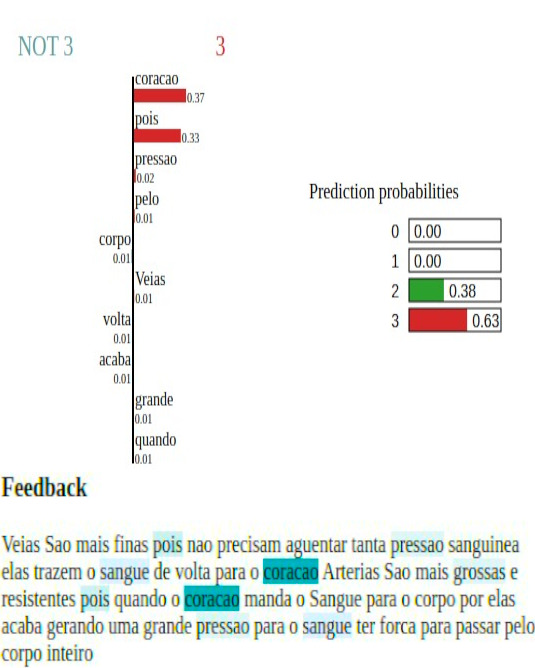
\includegraphics[width=.75\textwidth]{figuras/exemplo/highlight.jpeg}
 \caption{Destaques nos principais termos da resposta do estudante \#1995 do \textit{PTASAG Atividade 46}.}
 \label{fig-highlight-46}
\end{figure}

Como é exposto na Figura \ref{fig-highlight-46}, os termos \textit{coração}, \textit{sangue} e \textit{pressão} são destaques dessa resposta. Porém, os termos poderiam ser encontrados nas demais respostas. Por isso, foi identificado que o contexto apresenta 63\% de correlação com demais menções que receberam nota 3. Um segundo modelo, também em níveis textuais, extrai o conteúdo chave, de acordo com os tópicos mencionados por nível de nota. Nesse nível aplica-se LDA \cite{hoffman2013} no reconhecimento da composição de nota, ou seja os termos que em tese são essenciais para receber cada uma das classes. O LDA é uma técnica que aplica estatística descritiva para equivalência parcial dos dados. Nesse caso, a identificação da compatibilidade vetorial entre os textos que compõem um determinado nível de nota \cite{sahu2020}. Portanto, os dois são complementares. Enquanto o primeiro observa cada resposta pela perspectiva da avaliação, o segundo realiza o oposto. 

Apesar do acompanhamento da dinâmica do sistema no processo avaliativo, é complexo ao sistema identificar padrões coerentes de resposta. Para isso, utiliza-se o quadro de \textit{rubrics} para representar o modelo avaliativo elaborado pelo sistema em conjunto com o professor. O quadro de \textit{rubrics} é um modelo de caracterização do processo avaliativo conforme o modelo de resposta esperado para cada nota. Após o processo avaliativo, este torna-se um descritor, determinando na perspectiva dos estudantes quais foram as principais características elencadas para cada nota. Na Tabela \ref{tab-rubrics-exemplo} há um exemplo do quadro de \textit{rubrics} para a nota 3 da \textit{Atividade 46}.

\begin{table}[!h]
\centering
\caption{Tabela de \textit{rubrics} para as duas notas encontradas na atividade exemplo e as respostas mais alinhadas com as palavras selecionadas pelo LDA.}
\label{tab-rubrics-exemplo}
\footnotesize
\begin{tabular}{ p{2cm} | p{14cm}}
\multicolumn{2}{l}{\textbf{PTASAG : Atividade 46}} \\ \hline
\multicolumn{2}{c}{\textbf{Nota: 3}} \\ \hline 
\multicolumn{2}{l}{\textit{T{\'o}picos: arterias coracao corpo levam pressao rico sangue veias}} \\ \hline
 \# & Exemplos \\ \hline
19 & Veias \textit{levam} o \textit{sangue} para o \textit{coracao} e as \textit{arterias} \textit{levam} o \textit{sangue} do \textit{coracao} As \textit{veias} sao mais finas e as \textit{arterias} sao grossas e resistentes\\ \hline
78 & As \textit{veias} \textit{levam} \textit{sangue} ate o \textit{coracao} elas nao aguentam muita \textit{pressao} As \textit{arterias} \textit{levam} o \textit{sangue} do \textit{coracao} para o resto do \textit{corpo} pois aguentam maior \textit{pressao} e sao maiores\\ \hline
242 & As \textit{veias} \textit{levam} \textit{sangue} do \textit{corpo} para o \textit{coracao} onde ele possa ser bombeado novamente para o \textit{corpo} As \textit{arterias} saem do \textit{coracao} tornando se cada vez mais finas esses vasos \textit{levam} o \textit{sangue} nutrientes e oxigenio do \textit{coracao} para os tecidos\\ \hline
328 & As \textit{arterias} transportam o \textit{sangue} que sai do \textit{coracao} inicialmente \textit{rico} em O2 as diversas partes do \textit{corpo} as \textit{veias} recolhem esse \textit{sangue} \textit{rico} em CO2 e \textit{levam} de volta para o \textit{coracao} As \textit{arterias} possuem paredes mais grossas e as \textit{veias} possuem valvulas que impedem o \textit{sangue} de voltar\\ \hline
372 & As \textit{veias} \textit{levam} \textit{sangue} do \textit{corpo} ao \textit{coracao} e as \textit{arterias} do \textit{coracao} ao \textit{corpo} Alem disso as \textit{arterias} sao mais grossas que as \textit{veias} para suportar \textit{pressao}\\ \hline
444 & As \textit{veias} realizam o transporte do \textit{sangue} venoso \textit{rico} em CO2 no sentido do \textit{corpo} para o \textit{coracao} Ja as \textit{arterias} carregam o \textit{sangue} \textit{rico} em O2 do \textit{coracao} para o \textit{corpo} Alem disso as \textit{arterias} sao mais grossas que as \textit{veias} pois tem que aguentar a \textit{pressao} exercido pelos batimentos cardiacos que bombam o \textit{sangue}\\ \hline
456 & As \textit{arterias} sao vasos sanguineos responsaveis por conduzir o \textit{sangue} para fora do \textit{coracao} carregando \textit{sangue} artereal \textit{rico} em O2 As \textit{veias} sao responsaveis por conduzir o \textit{sangue} proveniente dos tecidos para o \textit{coracao} onde e \textit{rico} em CO2 e carrega \textit{sangue} venoso\\ \hline
479 & As \textit{veias} \textit{levam} o \textit{sangue} dos tecidos para o \textit{coracao} e possuem baixa \textit{pressao} ja as \textit{arterias} possuem alta \textit{pressao} e \textit{levam} \textit{sangue} do \textit{coracao} para o \textit{corpo}\\ \hline
\hline
\end{tabular}
\end{table}

Na Tabela \ref{tab-rubrics-exemplo} foram coletados os tópicos mais relevantes em cada uma das categorias para destacar os principais termos das respostas. No exemplo a resposta nota 3 fica evidente. Esta deve citar a relação entre o \textit{corpo} e o \textit{coração}, com a \textit{pressão} \textit{arterial} levando o sangue, e retornando pelas \textit{veias}. Então, a função do \textit{rubrics} é definir os padrões de resposta do sistema e, adicionalmente, criar relatórios que expliquem o formato avaliativo em apoio ao professor.
